%!TEX program=lualatex
%!TEX options=-synctex=1 -interaction=nonstopmode -halt-on-error "%DOC%.tex"
\documentclass[11pt,pdfa,lastpage,minititle]{MishoNote}
\title{Remarks on Grading Policy and Conventions in Sho's Grading}
\author{Sho Iwamoto}
\hypersetup{
  pdflang={en-US},
  pdfauthortitle={Assistant Professor, National Sun Yat-sen University},
  pdfsubject={Notes on Sho's grading conventions},
  pdfcontactemail={iwamoto@g-mail.nsysu.edu.tw},
  pdfcontacturl={https://www2.nsysu.edu.tw/iwamoto/},
  pdfcaptionwriter={Sho Iwamoto},
  pdfcopyright={2023–2025 Sho Iwamoto},
  pdflicenseurl={https://www2.nsysu.edu.tw/iwamoto/},
}
\renewcommand\thesubsection{\arabic{subsection}.}
\begin{document}
\maketitle

This document outlines the grading policies for exams, quizzes, and assignments in Sho's lecture courses at National Sun Yat-sen University (NSYSU).
These policies apply only to Sho’s courses and not to those of other faculty members.

\subsection*{Overview}
The grading policy for Sho's courses at NSYSU should follow the \hrefFN{https://regs.nsysu.edu.tw/rule/rul_vie?rul=20190816111934}{university regulation}.
The method of calculating the final grade is stated in the syllabus (``Administrative Information'') of each course, which is designed with the following standards:
\begin{miniitemize}
  \item $\mathbfup{A+}$ for ``performance gone beyond Sho's expectation'',
  \item $\mathbfup{B-}$ for ``partial achievement of the lecture goals with some shortcomings'', and
  \item $\mathbfup{C-}$ for ``achievement of the minimum lecture goals but with major shortcomings''.
\end{miniitemize}
\OutputNote


\subsection*{Policy on the return of answer sheets}
In principle, Sho will not return answer sheets of mini tests, quizzes, or exams.
This is because Sho believes that returning exam sheets does not improve students' learning:
\begin{itemize}
  \item Sho wants students to develop as independent thinkers, not to rely on the ``truth'' given by authority. Hence, Sho does not want to give them ``correct answers.''
  \item Returning answer sheets consumes significant time of Sho, but does not improve student learning. Even if Sho returns the answer sheets, students usually focus only on their scores, not on the content. Motivated students review exams regardless of whether sheets are returned, while unmotivated students do not review in either case.
  \item The primary purpose of exams is to evaluate achievement, not to provide feedback or promote further learning. If students need advice or feedback, they should ask before the exam.
  \item According to NSYSU regulations, faculty are not required to return answer sheets.
\end{itemize}
 However, the following cases are exceptions:
\begin{itemize}
  \item For a ``mini test'', which is designed for Sho to provide feedback on student answers, rather than to evaluate achievement. Sho will give feedback comments so that students can recognize shortcomings in their discussion and writing.
  \item In fall-semester lectures targeting first-year students, who are still ``kids'' in their first semester and not yet mature enough to behave as independent thinkers.
  \item After an exam, if a student reworks it, produces revised answers, and submits them during an in-person meeting (e.g., office hours).
\end{itemize}

\subsection*{Mark Style}
Sho's feedback on your answers will be given using the following mark style:

\begin{DownPara}
\begin{tabbing}
  \kern1.3em\=\kern1.3em\=\kern4.5em\=\kern7em\=\kill
  \JA{○}\>: correct\\
  \JA{○}\kern-0.7em \raise0.3ex\hbox{\small\textsf s}\>: correct but mishandling of significant figures.\\
  \JA{×}\>: incorrect\\
  \JA{△}\>: partial mark (with a number $n$ $\to$ $n$\JA{折})\addnote{For $1\le n\le 9$, $\text{(full mark)}\times0.1n$. For $10\le n\le99$, $\text{(full mark)}\times0.01n$.}.\\[.5em]
  \textsf{ACCEPT}: a problematic answer but accepted as a correct answer.\\[1em]


  \fbox{\makebox[1.8em]{\textsf{UM}}}\>\>: unit missing\\
  \fbox{\makebox[1.8em]{\textsf{UE}}}\>\>: unit handling error\\
  \fbox{\makebox[1.8em]{\textsf{UD}}}\>\>: unit duplication\\
  \fbox{\makebox[1.8em]{\textsf{DM}}}\>\>: direction missing\\
  \fbox{\makebox[1.8em]{\textsf{DE}}}\>\>: direction error\\
  \fbox{\makebox[1.8em]{\textsf{Dir}}}\>\>: direction missing/error\\
  \fbox{\makebox[1.8em]{\textsf{VE}}}\>\>: vector handling error\\
  \fbox{\makebox[1.8em]{\textsf{Exp}}}\>\>: insufficient explanation\\
  \fbox{\makebox[1.8em]{\textsf{Calc}}}\>\>: calculation error\\[1em]

  underline ending with \JA{┘}\>\>\>\>: correct claim for partial mark\\
  underline ending with a number\>\>\>\>: correct claim for partial mark indicated by the number\\
  underline ending with \JA{×}\>\>\>\>: incorrect claim\\[1em]

  wavy underline\>\>\>: critical issue (usually it leads you to a wrong answer)\\
  purple marker\>\>\>: English issue (tolerated)\\
  yellow marker\>\>\>: minor issue (tolerated)\\
\end{tabbing}
\end{DownPara}

\noindent
(Sample: For a two-second free fall of a 5\,kg object, find the final kinetic energy and average speed.)
\begin{center}
  \fbox{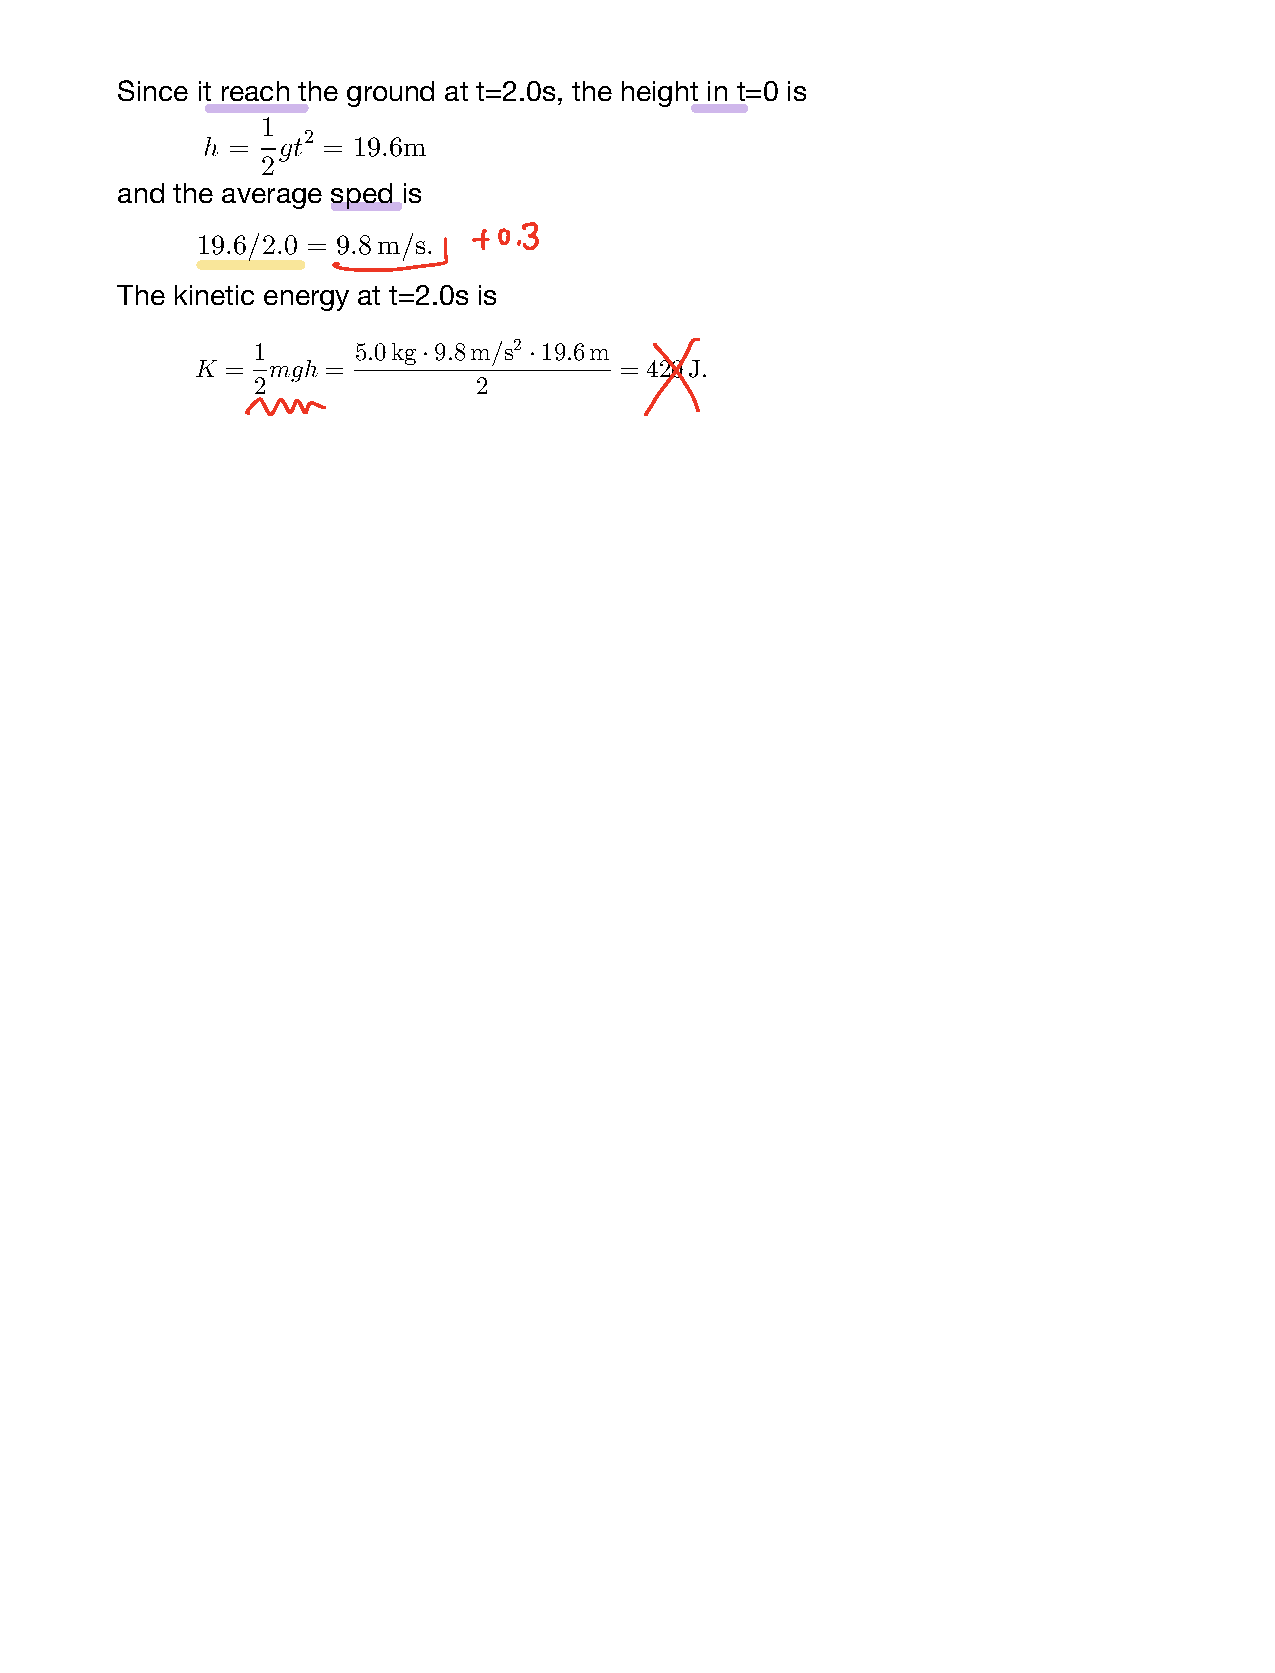
\includegraphics[width=0.6\textwidth]{grading_example.pdf}}
\end{center}

\OutputNote

\end{document}

